\chapter{Methodology}
% (diagram: data flow ; from input to output, everything in between; a paragraph on each module)
\section{Research paradigm: Action-Design-Research} 
As all of these items are conducted in a very agile approach, namely with \gls{ADR}, it is assumed that evaluation of tasks will take place immediately before each task was completed. There will be a strong focus on interviews and a constant exchange with experts. 

%%% 

\section{Development technique: Minimum Viable Product (MVP)}
The concept of a Minimum Viable Product (MVP) was first introduced by \citeauthor{Ries:2011:TheLeanStartUp} E. in \citeyear{Ries:2011:TheLeanStartUp} as a methodology for creating a 'Lean StartUp'. It aims at starting the learning process as early as possible through integrating early adopter's feedback.\cite{Lenarduzzi:2016:MVP}
\newline\newline
The Build-Measure-Learn loop is one of the core principles in 'Lean StartUp' which allows entrepreneurs to learn whether to give up or persevere with a current build \cite{Lenarduzzi:2016:MVP}. This build is usually defined as a MVP. The author \citeauthor{Ries:2011:TheLeanStartUp} E. describes an Minimum Viable Product as follows:
\begin{quote}
    "The MVP is that version of the product that enables a full turn of the Build-Measure-Learn loop with a minimum amount of effort and the least amount of development time."\cite{Ries:2011:TheLeanStartUp}
\end{quote}
However, a MVP is still far from being complete, on the contrary, it requires additional effort during building as its outcomes will be presented to potential customers and its feedback needs to be measurable. \cite{Ries:2011:TheLeanStartUp}
\newline\newline

\textbf{Paragraph -> How does MVP manifest itself in this thesis?}

    
    
%%%%%%%%%%%%%%%%%%%%%%%%%%%%%%%%%%%%%%%%%%%%%%%%%%%%%


\section{Methods}	
\begin{figure}[H]
  \begin{center}
  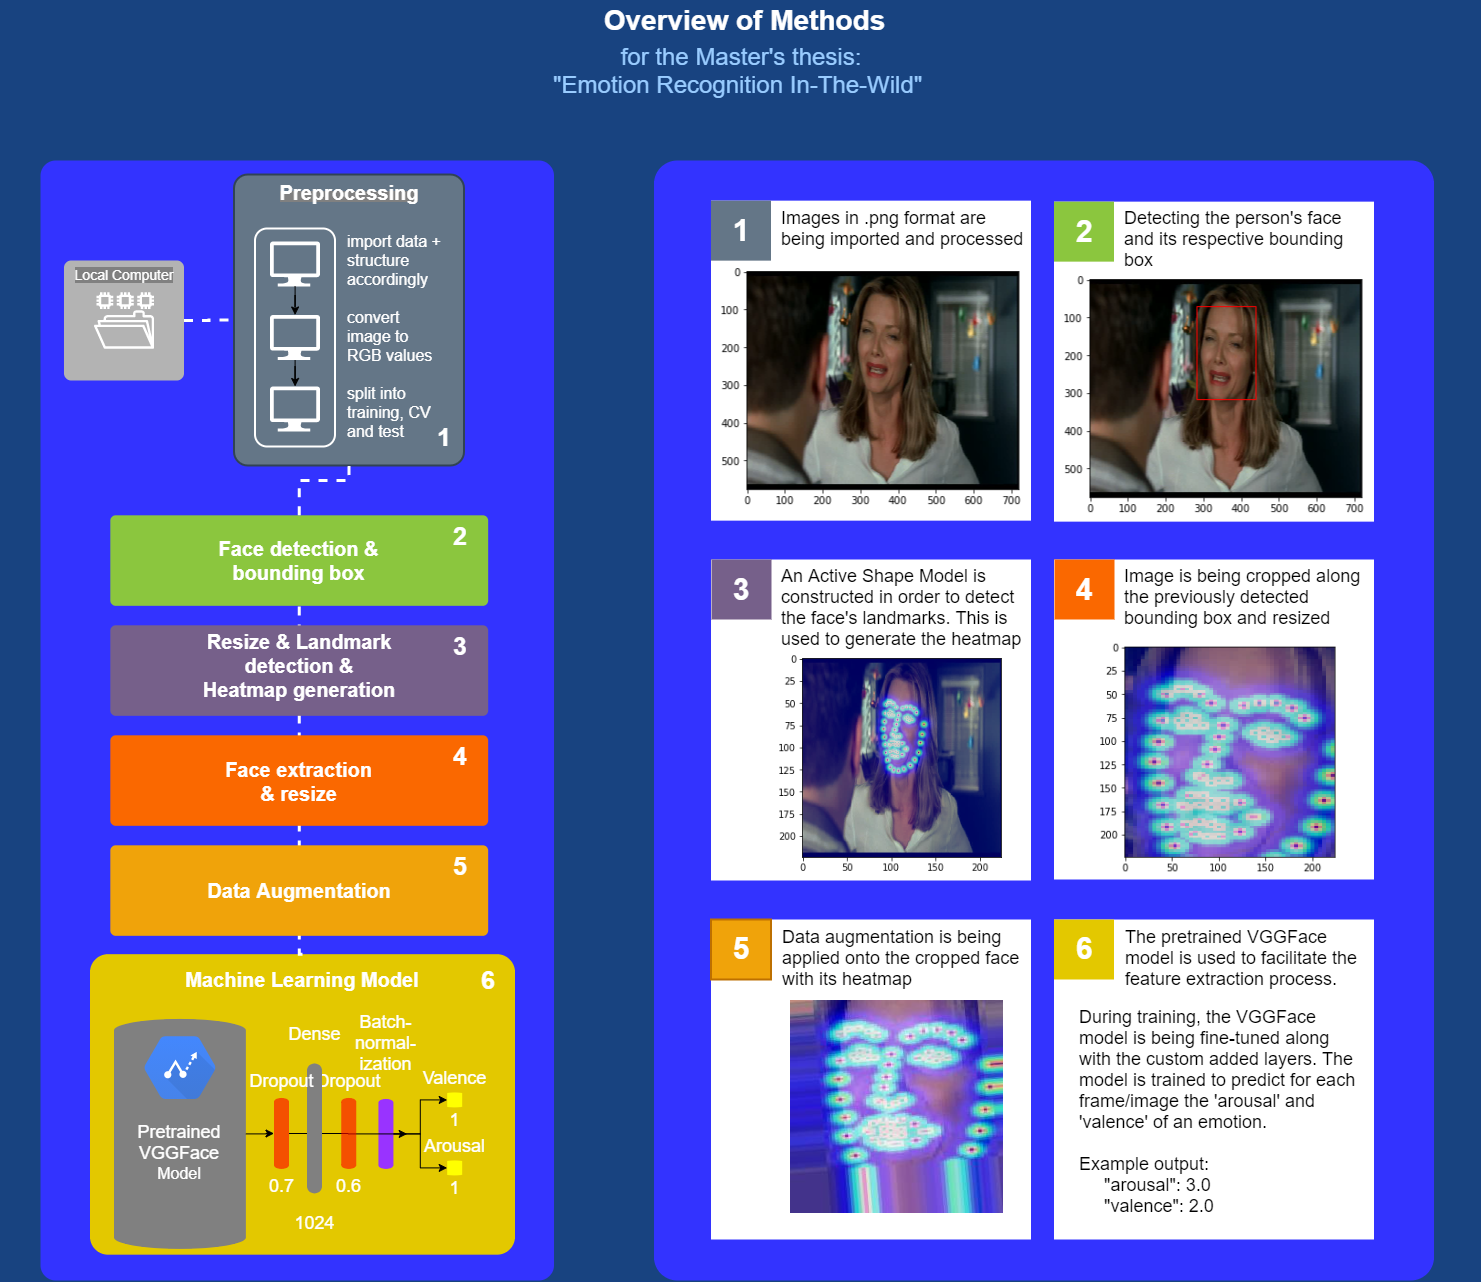
\includegraphics[angle=90, width=1.0\textwidth]{Figures/DataFlow_Diagram.png}
  \caption{Overview: Machine Learning Model - Components}
  \label{fig:MachineLearningModelComponents}
  \end{center}
\end{figure}

Approach:
1. Face detection
using MTCNN (Simultaneous face detection, face alignment, bounding boxing and landmark detection)\cite{Brownlee:2019:VggFace2HowToFaceRec}

2. Highlighting faces
draw the bounding box in an image and plot it\cite{Brownlee:2019:VggFace2HowToFaceRec}

3. Face extraction
extracting the face according to the identified bounding box
\cite{Brownlee:2019:VggFace2HowToFaceRec}

4. Face recognition
Using the VGGFace pretrained Resnet50 model to recognize emotions (training + prediction)
\cite{Sharma:2018:RealTimeFacialExpression}


\subsection{Preprocessing}
\subsubsection{Data construction}
Firstly, before reading in the actual image data, data description files are being read and analyzed. These description files are located inside subfolders of the dataset, one file for each speaker.
After all these description files are being read in from the data structure, a list of all image-filenames and their respective labels for valence and arousal is created.
\newline\newline
These lists are then being shuffled for a better randomization and are then split into training and testing data. Hereby, 25 per cent of the part of the dataset that is read in (a small part is reserved for final prediction testing) is used as a validation set.
\newline\newline
Furhtermore, labels are preprocessed by splitting each value through the number 5, as the original data, which ranges from -5 to 5, needs to be resized to a range of -1 to 1 in order to fit the activation function of the final layer which is a tanh activation function.
\newline\newline
The last preprocessing step involves loading all the images, converting it into RGB values and then extracting the face while using the face detection techniques described in the next chapter. The cropped output image will have a shape of 224x224x3 and will be permanently saved so that this step doesn't have to be repeated each time the model is being trained. Furthermore, the model can then reach back to this array of extracted images and directly use them to train or finetune the model.


\subsection{Face detection}
Made use of MTCCN to detect faces in images, set a bounding box and extract the face of an image.\cite{Zhang:2016:MTCCN}

1. Read the image, convert it to gray-scale and save it.
2. Read that gray-scale saved image, then detect face in it using HAAR cascade.
3. Crop the image to the detected face and resize it to 350*350 and save the image.
4. Read that processed cropped-resized image, then reshape it and normalize it.
5. Then feed that image to VGG-16 and create bottleneck features of that image and then reshape it.
6. Then use our own model for final prediction of expression.\cite{Sharma:2018:RealTimeFacialExpression}

\subsection{Finetuning VGGFace}

1. Pretrained VGGFace Model
—In this paper, we introduce a new large-scale face dataset named VGGFace2. The dataset contains 3.31 million images of 9131 subjects, with an average of 362.6 images for each subject. Images are downloaded from Google Image Search and have large variations in pose, age, illumination, ethnicity and profession (e.g. actors, athletes, politicians). 
The dataset was collected with three goals in mind: (i) to have both a large number of identities and also a large number of images for each identity; (ii) to cover a large range of pose, age and ethnicity; and (iii) to minimise the label noise. We describe how the dataset was collected, in particular the automated and manual filtering stages to ensure a high accuracy for the images of each identity. To assess face recognition performance using the new dataset, we train ResNet-50 (with and without Squeeze-andExcitation blocks) Convolutional Neural Networks on VGGFace2, on MS-Celeb-1M, and on their union, and show that training on VGGFace2 leads to improved recognition performance over pose and age. Finally, using the models trained on these datasets, we demonstrate state-of-the-art performance on the face recognition of IJB datasets, exceeding the previous state-of-the-art by a large margin.\cite{Cao:2018:VGGFace2}
\newline\newline
The VGGFace model is at foremost used to extract features from the data and allow the custom built top layers to learn the connection between extracted features and desired output (=label). Additionally, it is also being finetuned, which means that is being adapted to the current challenge at hand. This is necessary because originally, the VGGFace model wasn't designed nor trained to be used for Emotion Recognition challenges. Hence, the layers inside the VGGFace model are being trained with the current dataset and their desired output labels. This is called finetuning, as the model will be adapted to better fit this Emotion Recognition challenge.